\chapter{Automatic Music Transcription}

\emph{Automatic Music Transcription} (AMT) is the design of computational algorithm converting an acoustic musical signal into some form of musical notation, such as sheet music or MIDI files \cite{Benetos2019}. AMT is a subset of the broader field of \emph{Music Information Retrieval}.

\section{Music Information Retrieval}

\emph{Music Information Retrieval} (MIR) is an interdisciplinary research field concerning extraction and inference of meaningful features from music, indexing of music using these features, and the development of different search and retrieval schemes \cite{Schedl2014}.

It involves several different scientific backgrounds such as: musicology, psychoacoustics, signal processing, informatics, and most recently, machine learning \cite{Wiki2024A}.

The acronym MIR (\emph{Musical Information Retrieval} was first used by Kassler in 1966, referring to a special-purpose programming language named MIR \cite{Kassler1966}. However, the term has significantly evolved since then.

\subsection{Examples of Problems in Music Information Retrieval}

The scope of Music Information Retrieval is very extensive. It includes but is not limited to:
\begin{itemize}
	\item \emph{Classification and Indexing}. The amount of available digital music is constantly increasing \cite{Orio2006} and there is a need to organize music data into categories in order to facilitate navigation through rich audio libraries, link related audio items or managing music archives.
	\item \emph{Audio Identification}. This task aims to identify a fragment of a given music recording under conditions of recording noise or other distortions. A well-known system for this purpose is \emph{Shazam}. A variant of this task is \emph{query by humming}, where a user hums or sings a melody, and the system recognizes the corresponding song \cite{Schedl2014}.
	\item \emph{Measuring Music Similarity}. This involves comparing different music pieces to determine their similarity. Analysis may include melody, harmony, rhythm, and lyrics, aiding in genre classification, mood-based recommendations, and identifying cover songs or similar musical styles \cite{Berenzweig2003}.
	\item \emph{Instrument/vocal recognition and separation}. The most general expression of the problem is to identify and separate each instrument from a given audio sample. A specific application is separating a vocal track from a full song.
	\item \emph{Recommendation Systems}. Certain music systems propose a list of music pieces (usually \emph{playlists}) based on user musical preferences with some parameters involved: \emph{accuracy}, \emph{diversity} or \emph{serendipity} (a measure how surprising a recommendation is) \cite{Schedl2014}.
	\item \emph{Audio Transcription}. In this task, audio recordings are converted into a written or symbolic form, such as sheet music or MIDI files. This involves detecting and notating various elements like pitches, rhythms, and possibly lyrics from the audio signal.
\end{itemize}

Our primary interest lies in the last area, audio transcription, which will be the focus of the next section.

\subsection{Sources of Music Information}

While the general scope of tasks and problem in Music Information Retrieval is very broad, the information can primarily be sourced from two categories of music representation: \emph{audio-based} and \emph{symbolic}. These two primary modes of representing music information have been discussed in detail in the preceding chapter.

Besides the two previously mentioned ways of music representation, there is also a bibliographic source of information. That includes: title, composer/arranger/performer, publisher, publication date, and sometimes additional information such as the date of a recording, information about the label publishing, catalog numbers, or music categorization by genre or style. Such bibliographic details can be integral to certain MIR systems, offering a different dimension of information beyond the audio and symbolic representations.

\subsection{Music Facets}

There are many aspects of musics one wish to extract from. Downie lists a few aspects, though not mutually exclusive, that can be subject to Music Information Retrieval \cite{Downie2003}:
\begin{itemize}
	\item \emph{Pitch Facet}.
	\item \emph{Temporal Facet}.
	\item \emph{Harmonic Facet}.
	\item \emph{Timbral Facet}.
	\item \emph{Editorial Facet}.
	\item \emph{Bibliographic Facet}.
\end{itemize}

Extracting each of these facets involves distinct methodologies as they operate on different layers of musical information.

For instance, generating a complete score from a performance MIDI requires the extraction of pitch, temporal, and editorial facets. While pitch and temporal aspects are present in the MIDI stream, the underlying harmonic and temporal structures, such as key and time signature, are not explicitly present and must be inferred.

In case of pitch, even for a MIDI file, ambiguity is still possible. For example, a MIDI note represented by the number 73 could, depending on the musical context, be interpreted as either $\textrm{C}\sharp$ or its enharmonic equivalent, $\textrm{D}\flat$. Similarly, note lengths are usually not preserved. For instance, a pianist's hand movement between notes (unless playing \emph{legato}) typically shortens the actual length of a note compared to its notated duration in the score.

The list above mentioned by Downie is not exhaustive: music is a very multimodal phenomenon and it comes not only with an audio, but also text (lyrics), images (album covers and photographs of musicians) or gestures of performers \cite{Schedl2014}.

\section{Automatic Music Transcription}

As defined by Benetos et al. \cite{Benetos2019}, \emph{Automatic Music Transcription} (AMT) is \emph{the design of computational algorithms to convert acoustic music signals into some form of music notation}. Typically, the input of an AMT system is a raw audio signal, encoded in one of common audio format, whether lossless (like WAVE, AIFF, FLAC) or compressed (such as MP3, AAC, or Ogg). The output of AMT systems varies and depends on specific use cases.

Regardless of the final output form, the general AMT task is a multi-staged process involving several different subtasks:
\begin{enumerate}
	\item Instrument recognition and separation
	\item (Multi-)pitch estimation
	\item Note onset and offset detection
	\item Beat and rhythm tracking
	\item Interpretation of dynamics
	\item Interpretation of instrument articulations
	\item Score typesetting
\end{enumerate}

AMT systems may focus on addressing only a subset of these problems, meaning not all stages are necessarily involved in every AMT task. Therefore, AMT should be viewed not as a singular task but as a class of various tasks. Often, the audio sample may be pre-processed into an intermediate form, such as a MIDI stream, before being subjected to further AMT processing.

\subsection{Application of Music Transcription}

AMT systems can be applied to facilitate a variety of routine tasks that musicians would do manually otherwise.

Benetos et al. (2013) highlights that one of \emph{the most immediate application of automatic music transcription is for allowing musicians to record the notes of an improvised performance in order to be able to reproduce it} \cite{Benetos2013}.

These systems can significantly aid in the learning process for individuals wishing to practice songs for which published scores are either unavailable or hard to access. These systems also may speed up the process of composing, when the tedious task of transcribing recordings is no longer necessary. The latter is the promise of performance MIDI to score transcription systems.

\subsection{Levels of Music Transcription}

Music transcription can be classified into four distinct levels: \emph{frame-level}, \emph{note-level}, \emph{stream-level}, and \emph{notation-level}, each with its unique purposes and challenges \cite{Benetos2019}.

\subsubsection{Frame-level Transcription}

\emph{Frame-level transcription}, also known as \emph{multi-pitch estimation} (MPE), involves estimating the pitch of notes at the level of individual samples (or frames), treated independently for each frame \cite{Bhattarai2023}. This form of transcription may be conducted under the assumption of either monophonic or polyphonic instrumentation, with the latter being more complex.

The outcome is a partial function (or a set of such functions) $f\colon I\to\mathbb{R}_{>0}$ where for each point of time $x\in I$ a frequency is assigned. Additionally, frame-level transcription often includes sound energy estimation.

This level of transcription is vital for pitch-correction tools such as \emph{Melodyne}. However, this level of transcription fails to capture a broader context of music structure.

\subsubsection{Note-level Transcription}

\emph{Note-level transcription} is one abstraction layer higher than frame-level transcription. It aims to estimate an entire note entity, recognize a note's pitch within a note onsets and offset. It often includes determining note velocities.

One possible format of the output of note-level transcription is a MIDI stream.

\begin{figure}[ht!]
\centering
\begin{tabular}{>{\centering\arraybackslash} m{0.05\textwidth} >{\centering\arraybackslash} m{0.95\textwidth}}
1 & \includesvg[width=0.9\textwidth]{images/pitch_estimation.svg}\\
2 & \includesvg[width=0.9\textwidth]{images/pitch_notes.svg}
\end{tabular}
\caption[A frame-level and note-level transcription of a vocal audio sample.]{A frame-level (1) and note-level (2) transcription of a vocal audio sample. The \emph{CREPE} algorithm has been used for a monophonic pitch estimation \cite{Kim2018}, and \emph{CREPE notes} for note quantization \cite{Riley2023}. Frequency instability leads to misaligned pitch attribution on a note-level transcription.}
\end{figure}

\subsubsection{Stream-level Transcription}

\emph{Stream-level transcription}, also known as \emph{multi-pitch streaming} (MPS), involves grouping estimated pitches or notes into separate streams, typically corresponding to individual instruments \cite{Bhattarai2023}. On that level of transcription, multi-pitch estimation is not sufficient as distinguishing different instruments is needed. The process of instrument differentiation is in fact a clustering problem.

Instruments differ in their timbres, or tone colors, which is the perceived quality of sound that makes two instruments sound distinct even when they play the same pitch at the same energy level. The timbre largely depends on an instrument's harmonic series and its variation over time (the envelope). This is merely a simplification: not all sounds conform to harmonic series representations; for example, noise or most percussion instruments are exceptions, though tonal instruments are generally well-described by harmonic series \cite[p.~27--28]{Sethares2005}.

Duan et al. (2014) defines the streaming tasks as: \emph{the clustering objective is to maintain timbre consistency, based on the assumption that sound objects coming from the same source have similar timbre} \cite{Duan2014}. Notes coming from the same instrument are expected to have similar timbre characteristic. Depending on the method, the number of instrument clusters may or may not be specified beforehand.

The timbre of an instrument is not static and can vary based on several factors, including:
\begin{itemize}
	\item The method and force of inducing vibration. For instance, a violin emits different sounds based on the bowing technique, and a piano's sound quality changes with the force applied to the keys.
	\item The fundamental frequency. The harmonic series of an instrument varies with the played note, often resulting in different overtone distributions in lower and higher registers.
	\item Playing technique. The way a musician produces sound can significantly affect timbre. On wind instruments, for example, variations in embouchure, tonguing, and breath control can create diverse timbral effects.
\end{itemize}

The timbre clustering becomes particularly challenging when similar but distinct instrument are played simultaneously, and their harmonic series are overlapping.

\subsubsection{Notation-level Transcription}

\emph{Notation-level transcription} is the process of converting audio recordings into a traditional music notation or a score \cite{Bhattarai2023}. This process transforms the musical content into a structured format as outlined in the previous section on \emph{Sheet Music}.

Besides the musical content, that is notes and rests, notation-level transcription involves assigning other various musical elements:
\begin{itemize}
	\item Instruments are organized by separate staves. Each instrument needs to be recognized and appropriately organized within the score.
	\item Tempo markings are usually indicated at the beginning of a piece but may vary throughout the composition.
	\item Clefs are used to suggest the pitch range of the voice or instrument. For instruments with a wide pitch range, such as the piano, the clef may change during the piece.
	\item Time signatures are essential, with the most common default being $\lilyTimeSignature{4}{4}$. While the time signature generally remains consistent across instruments, it can vary within a piece.
\end{itemize}

Some notation-level transcription methods might come with certain limitations and not provide all these elements. For instance, they might default to using the $\textrm{C}$ major treble clef and the common $\lilyTimeSignature{4}{4}$ time signature for all staves, regardless of the song's actual key or time signature. Some methods may also assume that a single instrument is being played.

\subsection{Stages of Music Transcriptions}

As previously discussed, the general transcription is a complex task consisted of several steps.

Assume we have a raw audio signal containing a recording of music. For the sake of simplicity, let us consider a raw audio signal containing a recording of music from a single polyphonic instrument such as piano or guitar.

In order to retrieve notes from the recording, usually the audio signal is converted to a spectrogram. This representation allows both pitch and energy estimation.

The transcription involves three challenges:
\begin{itemize}
	\item \emph{Detecting Pitch Frequencies}. Notes usually produce a series of harmonics – multiples of a fundamental frequency – each with varying energy levels that change over time. Additionally, the fundamental frequency itself may fluctuate due to vibration and glide. This task is further complicated by the limited frequency resolution of the short-time Fourier transform.
	\item \emph{Recognizing Time Onsets and Offsets}: Identifying when a note begins and ends is straightforward in monophonic music but becomes significantly more complex in polyphony, where multiple notes are often played with slightly different timings, and their envelopes overlap with each other. As in the previous task, time resolution of the short-time Fourier transform is limited as well.
	\item \emph{Measuring Note Velocity}. Notes can be played with different energy, resulting a sound with different amplitude. Accurately assigning velocity to each note is difficult, especially when notes have overlapping harmonic series and energy attribution becomes ambiguous. Also a limited resolution of a Fourier transform contribute to this effect.
\end{itemize}

There are different strategies to overcome these obstacles. Assuming that there is only one instrument playing, these are covered by note-level transcription.

The outcome of this process is a \emph{performance MIDI} or a \emph{MIDI stream}, comprising a sequence of notes characterized by four features: pitch, note onset, duration, and velocity.

A MIDI stream lacks information about the underlying music structure. More specifically, certain vital score elements are still yet to be determined: time signatures, key signatures, voicing (e.g. hand part assigning for piano recordings). Moreover, notes and rests need to be quantized into standardized lengths (e.g., whole notes $\wholeNote$, half notes $\halfNote$, quarter notes $\quarterNote$, etc.).

The final stage is notation-level transcription: transforming the performance MIDI into a scored format. This involves imposing the structure mentioned above and then rendering the score in a specific music data format.

\begin{figure}[ht!]
\centering
\begin{tabular}{>{\centering\arraybackslash} m{0.05\textwidth} >{\centering\arraybackslash} m{0.95\textwidth}}
1 &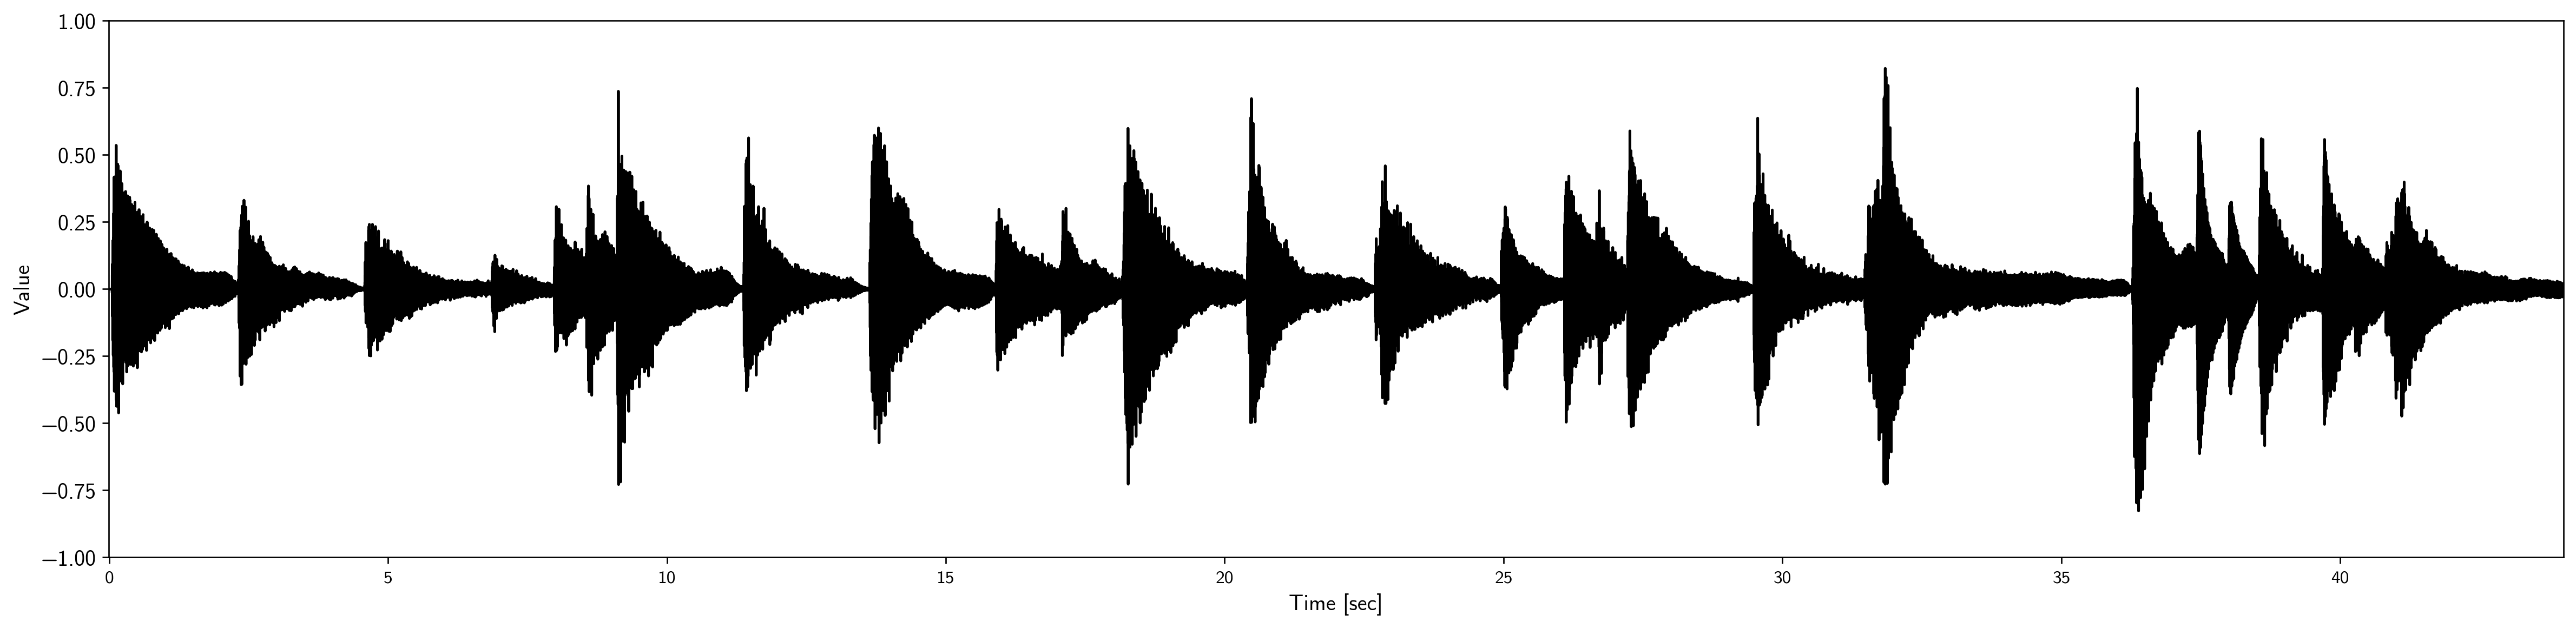
\includegraphics[width=0.9\textwidth]{images/amt_0.png} \\
2 &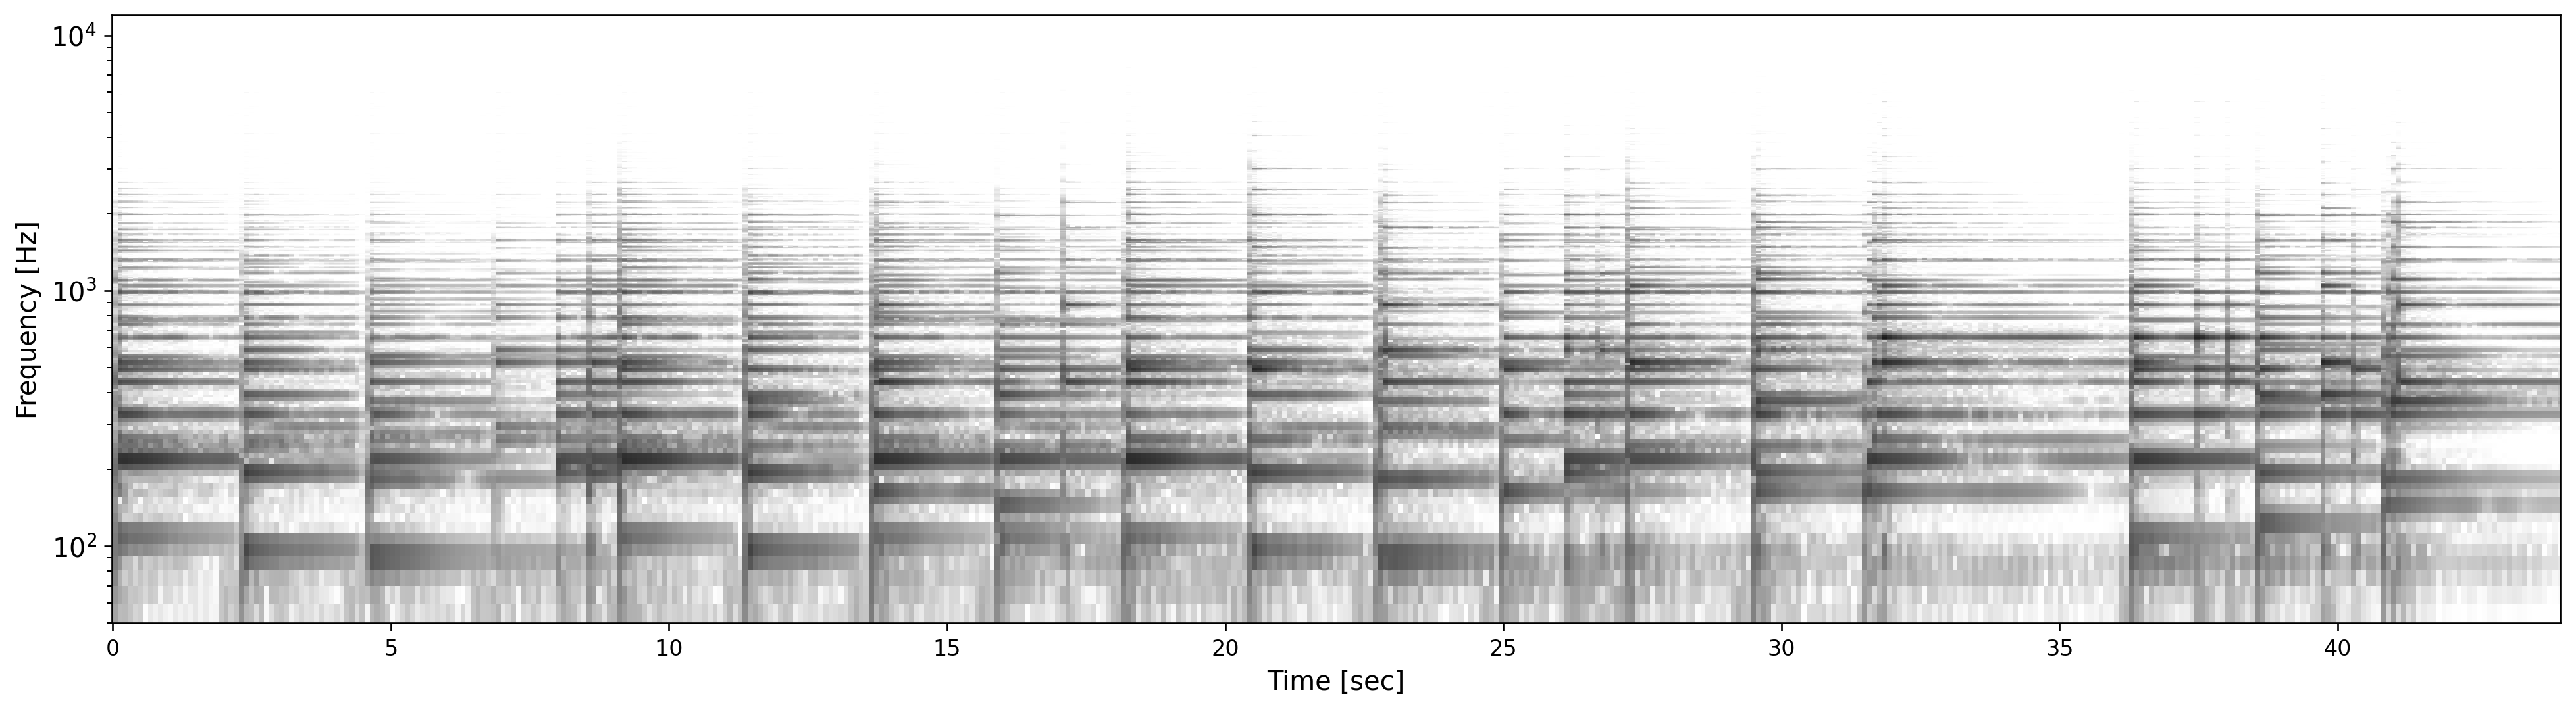
\includegraphics[width=0.9\textwidth]{images/amt_1.png} \\
3 &\includesvg[width=0.9\textwidth]{images/piano_roll.svg} \\
4 &\includesvg[width=0.9\textwidth]{images/amt_gen.svg}
\end{tabular}
\caption[An example of an Automatic Music Transcription task on a concrete piano recording.]{An example of an Automatic Music Transcription task on a concrete piano recording. First, the audio sample (1) is transformed to a spectrogram (2) using the short-time Fourier transform, from which notes are retrieved. The result of that process is a sequence of a MIDI stream (3) for which the other aspects of music score are determined (here: clefs, key signature, time signature, tempo marking) and transcribed to a final score (4).}
\end{figure}

This stage of audio transcription is the main focus of this work, concerning mostly on digital piano recordings. From now on we will assume that the performance MIDI is given, either retrieved from the audio signal, or recorded directly via some MIDI instrument. However, we do not care about the visual aspects of the score, only its content. The more precise definition of \emph{content} will be formalized in the next fragment.

\subsection{Performance MIDI to Score Transcription}

Let us review basic assumptions of the performance MIDI to score process. In this section, we follow the name convention of Liu et al. (2022), the authors of the main performance MIDI to score model discussed \cite{Liu2022}. However, a few adjustments have been made.

\subsubsection{Performance MIDI Encoding}

The input performance MIDI may be encoded as a sequence $\mathbf{X}=\left\{p_i,o_i,d_i,v_i\right\}_{i=1}^N$ of a variable length $N$, of four features: \emph{pitch} $p_i$ (an integer from the range $0$ to $127$), \emph{onset} $o_i$ being a positive real number, \emph{duration} $d_i$, also a positive real number, and \emph{velocity} $v_i$, an integer from range $0$ to $127$. The velocity may be further normalized to a rational number from the unit interval. We assume also that the sequence is sorted firstly by the onset, and secondly by the pitch in the ascending order.

The encoding of a performance MIDI is in fact a two-dimensional tensor. We will call such encoding also a performance MIDI, when no confusion arises.

\subsubsection{Music Score Encoding} \label{music_score_encoding}

In this section, we define a music score in terms of the essential elements it needs to encode. The output of our automatic transcription method focuses solely on the abstract elements of a score, entirely disregarding the visual layout.

These elements include:
\begin{itemize}
	\item \emph{Tempo}, quantized as an integer within the range of $0$ to $200$. Practically, only values above $30$ are  expected.
	\item \emph{Downbeats} and \emph{beats}, marking sections of each measure\footnote{The downbeat is the first beat of a measure.}. This segmentation helps convert a rhythmically unstructured MIDI into structured measures and identify the initial beats of these measures. Both elements are binary.
	\item \emph{Musical onsets}, indicating the start of notes in terms of quantized beat divisions. Whole integers correspond to notes beginning on a downbeat.
	\item \emph{Note values}, representing durations as quantized lengths (e.g., $1$ for a whole note, $\frac{1}{2}$ for a half note). However, note values are categorical.
	\item \emph{Key signature}, chosen from one of $12$ possible scales: $\textrm{C}$, $\textrm{C}\sharp$, $\textrm{D}$, \ldots, $\textrm{A}\sharp$, $\textrm{B}$, each treated as a separate category.
	\item \emph{Time signature}, consisting of a numerator and denominator. Since there are only several common time signatures, one can narrow down the choice of possible values: $0$, $2$, $3$, $4$ and $6$ for the numerator, and $0$, $2$, $4$ and $8$ for the denominator. The value $0$ stands for other values.
\end{itemize}

Musical onsets, note values, and even key/time signatures may be assigned for each note. Beats and event downbeats may not come without notes and their prediction cannot be done on the note level.

Since we expect only piano recordings, we also aim to differentiate between left and right hand parts, represented as two staves with treble and bass clefs, respectively. This assignment is binary.

Note that pitch values are derived directly from the input. Articulation and dynamic markings are not considered within the scope of the model proposed by Liu et al. (2022).

To summarize, the output score $\mathbf{Y}$ can be represented as a pair of two tensors $\left(\mathbf{Y}_b, \mathbf{Y}_n\right)$:
\begin{itemize}
	\item The beat tensor $\mathbf{Y}_b = \left\{t_j, db_j\right\}_{j=1}^B$ encapsulates the real times $t_i$ of beats, along with a binary downbeat classification $db_i$.
	\item The note-level tensor $\mathbf{Y}_n=\left\{mo_i, nv_i, h_i, tn_i, td_i, k_i, tem_i\right\}_{i=1}^N$ where $mo_i$ is quantized music onset, $nv_i$ is the note value, $h_i$ indicates the hand part of a note (left or right), $tn_i$ and $td_i$ are time signature numerators and denominators, $k_i$ is the key signature, and $tem_i$ is the BPM represented as an integer. All values are categorical.
\end{itemize}

The objective of performance MIDI to score automatic transcription is to find a good enough function $\mathbf{X}\to\mathbf{Y}$. Further sections will be devoted to measuring the quality of the resulting score in order to define the \emph{good enough} part. 

\section{Challenges in the Transcription Task}

Before providing an overview of methods for MIDI to score conversion, it is essential to first understand the inherent challenges of the transcription task. We need to examine how a performance captured in a MIDI file deviates from traditional sheet music and identify the types of information that are lost in the process of translating between these two forms of musical representation.

Some challenges are directly related to the way musical data is encoded in the MIDI format, such as the issue of \emph{note spelling}\footnote{See the Section \ref{harmonic_equivalence} for the explanation.}. This leads to ambiguities that require further disambiguation through additional algorithms or human intervention.

Other challenges arise from the nature of musical performance itself and the variations that occur when a piece is interpreted and played. A live performance rarely, if ever, adheres strictly to the abstract representations of rhythm and timing found in traditional notation. Some vital aspects of the human performance are described in more detail in the next section.

\subsection{Common Transcription Problems}

Traditional music notation represents an idealized version of how a piece should be played. While it provides a structured framework for pitch, rhythm, dynamics, and articulation, it abstracts away from many performance nuances that are either too subtle, too variable or simply irrelevant to be captured in symbolic notation.

\begin{figure}[ht!]
\centering
\begin{tabular}{cc}a)
\includesvg[width=0.3\textwidth]{images/sonata_original_gen.svg}
 & b)\includesvg[width=0.6\textwidth]{images/sonata_performance_gen.svg}
\end{tabular}
\caption[An example of the imported performance MIDI of Chopin's \emph{Sonata No. 2, Op. 35, 2nd movement} ``as it is''.]{An example of the imported performance MIDI of Chopin's \emph{Sonata No. 2, Op. 35, 2nd movement} ,,as it is'': a) the original sheet, b) the imported performance MIDI without time/key signature assignment. Not only the actual durations render the sheet unreadable and impractical, but also introduce error resulting from note quantization. Notice that there is no hand separation.}
\label{chopin_sonata}
\end{figure}

These deviations can make the direct conversion of performance MIDI into readable sheet music difficult, as exemplified in Figure \ref{chopin_sonata}. Below, we will explore some of the most common transcription problems.

\subsubsection{Tempo}

MIDI files operate with a fixed tempo, or more precisely, a discrete set of tempo changes. A human performer, however, never aligns to the tempo perfectly, even in a course of a single measure.

In many cases, these deviations are deliberate. For example, a performer might slow down (\emph{rubato}) or sustain a note longer than notated (\emph{fermata}) for expressive purposes. While these nuances may sometimes be annotated in the score, it is not always the case, and even when marked, the precise nature of the tempo fluctuation is left to the performer’s interpretation. Performers have considerable freedom in determining the extent and suddenness of tempo changes, which MIDI struggles to represent accurately.

More importantly, performance MIDI files often do not reflect internal tempo structures, rendering the ticks-per-quarter-note parameter ineffective. This issue is further addressed in Section \ref{score-informed_midi_files}.

\subsubsection{Note duration}

In live performances, note durations often deviate from those specified in the score. Pianists, for example, tend to slightly shorten note lengths to prepare for the next note or chord.

In \emph{legato} playing, some notes may be overlapping and their actual length is a bit longer than indicated by the notation. This elongation is especially prominent in rapid, fluid passages. Conversely, \emph{staccato} notes, which are played with almost immediate release, are never denoted with actual expected time of playing. Traditional notation primarily indicates note boundaries, leaving the actual performed lengths to be interpreted by the pianist.

\subsubsection{Dynamics}

The traditional notation system offers a relatively limited palette of dynamic markings, ranging from \emph{pianississimo} ($\lilyDynamics{ppp}$) to \emph{fortississimo} ($\lilyDynamics{fff}$). Changes in volume over a phrase are marked by \emph{crescendo} ($\crescHairpin$) and \emph{diminuendo} ($\decrescHairpin$) symbols. Thorough centuries, the notation has been expanded and introduced new markings such as \emph{sforzando} (sfz) or \emph{subito forte} (sf).

The dynamics are not absolute, rather contextual and depending on the surrounding musical elements. Since these markings are guidelines, there is some room for interpretation by the performer.
	 	 
In contrast, MIDI format stores a concrete note velocity with 7-bit precision. As a rule of thumb, the following arbitrary classification is adopted:

\begin{table}[!ht]
\centering
\begin{tabular}{ccc}
    Dynamic              & Marking              & Velocity \\\hline
    \emph{pianississimo} & $\lilyDynamics{ppp}$ & 16       \\
    \emph{pianissimo}    & $\lilyDynamics{pp}$  & 33       \\
    \emph{piano}         & $\lilyDynamics{p}$   & 49       \\
    \emph{mezzo-piano}   & $\lilyDynamics{mp}$  & 64       \\
    \emph{mezzo-forte}   & $\lilyDynamics{mf}$  & 80       \\
    \emph{forte}         & $\lilyDynamics{f}$   & 96       \\
    \emph{fortissimo}    & $\lilyDynamics{ff}$  & 112      \\
    \emph{fortississimo} & $\lilyDynamics{fff}$ & 127
\end{tabular}

\caption[The dynamics table.]{The dynamics table.\missing}
\end{table}

While the MIDI format represents the dynamics numerically instead of symbolically, there is no direct translation of the actual note velocity to dynamics markings: these describe broader phrases rather than individual notes. An analysis is required to translate raw velocity data into meaningful dynamics guidelines.
	 
The standard transcription model does not handle dynamics explicitly. Experimental methods addressing this issue are discussed in Chapter \ref{experiments_and_improvements}.

\subsubsection{Harmonic Equivalence}\label{harmonic_equivalence}

As the MIDI file format does not distinguish enharmonically  equivalent pitches, we generally cannot solve the problem  of pitch spelling, that is assigning correct \emph{accidentals}: flats ($\flat$) or sharps ($\sharp$) \cite{Cambouropoulos2000}. For example, in keys like D major or G major, a MIDI note 66 is likely to be spelled as F$\sharp$, while the same pitch may function as G$\flat$ in keys such as E$\flat$ or B$\flat$ minor.

The ambiguity can be resolved through assigning the key signature, that is determining the key of the scale. This approach has been successfully used in \cite{Liu2022}.

\subsubsection{Voicing}

A \emph{voice} (or \emph{stream}) is defined as "a monophonic sequence of successive, non-overlapping musical tones" \cite{Karydis2007}. This notion can be broadened to any sequence of notes, whether monophonic or polyphonic, that is perceived as a single musical entity \ref{Cambouropoulos2008}.

\begin{figure}[ht!]
\centering
\includesvg{images/bach_fugue_gen.svg}
\caption[Four independent voices in the Fugue No.1 in C Major, BWV846 by J.S. Bach.]{Four independent voices in the Fugue No.1 in C Major, BWV846 by J.S. Bach.}
\end{figure}

A single MIDI track can be viewed as a collection of notes, and the MIDI format does not offer any levels of further subdivisions. Consequently, exporting a score to a MIDI file loses all information regarding the original voicing. For that reason in the case of piano music, it is common (but not guaranteed) to separate left-hand and right-hand notes into two tracks, corresponding to the two hands. Since there can be more voices than only indicated by the left and hand right (as the example above shows), the hand separation is a subset of a broader challenge of voice separation. For a related work in that matter, refer to \cite{Karydis2007}.
	
\subsection{Score-Informed MIDI files}\label{score-informed_midi_files}

As noted previously, performance MIDI files are generally not aligned to an internal MIDI tempo. One can correct a MIDI file by assigning the tempo so that every beat in the piece corresponds to the same number of ticks. This process effectively regularizes the performance by aligning it with the underlying metric structure of the music.

Grohganz et al. \cite{Grohganz2014} identify two types of MIDI files based on this alignment: \begin{enumerate}
	\item \emph{S-MIDI}: \emph{Score-informed} MIDI files, which have been aligned to a specific tempo, ensuring that the musical events correspond accurately to the beat structure.
	\item \emph{P-MIDI}: Unaligned \emph{performance} MIDI files, where the real tempo of the performance is unknown or inconsistent with the internal timing of the MIDI format. \end{enumerate}

\begin{figure}[ht!]
\centering
\begin{tabular}{cc}a)
\includesvg[height=1.25cm]{images/score_agnostic_gen.svg}
 & b)\includesvg[height=1.15cm]{images/score_informed_gen.svg}
\end{tabular}
\caption[An actual recording of a simple melody]{An actual recording of a simple melody: a) the score-agnostic recording with incorrectly quantized musical onsets not aligned with the MIDI tempo, b) the score-informed representation of the performance. Notice that the pickup measure is also correctly identified.}
\label{score_informed}
\end{figure}

The beat quantization problem may be thought as a process of converting a P-MIDI into a S-MIDI file.

Most musical software programs struggle to correctly import P-MIDI as they rely on the internal tick-based structure to interpret note onsets. Without accurate alignment to a tempo grid, the resulting transcription can appear rhythmically distorted, with notes placed in incorrect positions relative to the beat (see: Figure \ref{score_informed}). This makes beat quantization an essential step in the transcription of human-performed music.

\subsection{Summary of Steps}

In summary, the procedure of translating the raw performance MIDI to a score involves at least: \begin{itemize}
	\item note quantization, which consists of:
	\begin{itemize}
		\item recognizing the beat grid within the downbeats
		\item interpreting the musical onsets according to the grid
		\item assigning proper musical duration to notes	
	\end{itemize}
	\item assigning time signatures
	\item assigning key signatures
	\item separating independent voices (here: separating hands)
\end{itemize}

Each of these subtasks will be implemented as a separate module within the main model architecture.

\subsection{Limitations}

While AMT systems aim to convert performance data into a readable musical score, only a subset of musical elements is typically included in the generated output. Many nuances remain beyond the scope of current AMT systems, including the main model described here.

Key limitations include: \begin{itemize}
	\item {\bf Accents and articulation marks}: Elements such as \emph{staccato}, \emph{tenuto}, or accents are vital for conveying how each note should be played in terms of attack, duration, and emphasis. None of them are handled by presented AMT models.
	\item {\bf Pedalization}: While MIDI files capture pedal events, the transcription process does not typically translate these events into notated pedal marks. A human intervention is often needed to transform raw MIDI signals into a clean notation.
	\item {\bf Ornaments}: Grace notes, trills, mordents, and other ornaments add complexity to both performance and notation. As the MIDI does not distinguish special notes, all of such ornaments are shown as ordinary notes. To the author's knowledge, there is no model that attempts to transcribe performance recording recognizing ornaments.
	\item {\bf Dynamics and expression marks}: While note velocity can give a rough indication of dynamics, AMT systems do not capture more complex dynamic markings like crescendo, diminuendo, or sudden dynamic shifts. A partial work in that matter can be found in the Chapter \ref{experiments_and_improvements}.
	\item {\bf Clefs}: The changes in the clefs are not registered in a MIDI stream. Thus, it is not a task of the model to assign clefs \footnote{Musical software often interprets MIDI files and handles clef assignments for the user \missing.}. For simplicity, we may assume that the treble clef constantly corresponds to the right hand, while the left hand is governed by the bass clef.
	\item {\bf Phrasing}: The subtle shaping of musical phrases, which performers use to convey musical direction and intention. Common group indications like slurs are absent in the generated scores. \end{itemize}

This is, of course, by no means an exhaustive list.
